\documentclass[twoside]{book}

% Packages required by doxygen
\usepackage{fixltx2e}
\usepackage{calc}
\usepackage{doxygen}
\usepackage[export]{adjustbox} % also loads graphicx
\usepackage{graphicx}
\usepackage[utf8]{inputenc}
\usepackage{makeidx}
\usepackage{multicol}
\usepackage{multirow}
\PassOptionsToPackage{warn}{textcomp}
\usepackage{textcomp}
\usepackage[nointegrals]{wasysym}
\usepackage[table]{xcolor}

% Font selection
\usepackage[T1]{fontenc}
\usepackage[scaled=.90]{helvet}
\usepackage{courier}
\usepackage{amssymb}
\usepackage{sectsty}
\renewcommand{\familydefault}{\sfdefault}
\allsectionsfont{%
  \fontseries{bc}\selectfont%
  \color{darkgray}%
}
\renewcommand{\DoxyLabelFont}{%
  \fontseries{bc}\selectfont%
  \color{darkgray}%
}
\newcommand{\+}{\discretionary{\mbox{\scriptsize$\hookleftarrow$}}{}{}}

% Page & text layout
\usepackage{geometry}
\geometry{%
  a4paper,%
  top=2.5cm,%
  bottom=2.5cm,%
  left=2.5cm,%
  right=2.5cm%
}
\tolerance=750
\hfuzz=15pt
\hbadness=750
\setlength{\emergencystretch}{15pt}
\setlength{\parindent}{0cm}
\setlength{\parskip}{3ex plus 2ex minus 2ex}
\makeatletter
\renewcommand{\paragraph}{%
  \@startsection{paragraph}{4}{0ex}{-1.0ex}{1.0ex}{%
    \normalfont\normalsize\bfseries\SS@parafont%
  }%
}
\renewcommand{\subparagraph}{%
  \@startsection{subparagraph}{5}{0ex}{-1.0ex}{1.0ex}{%
    \normalfont\normalsize\bfseries\SS@subparafont%
  }%
}
\makeatother

% Headers & footers
\usepackage{fancyhdr}
\pagestyle{fancyplain}
\fancyhead[LE]{\fancyplain{}{\bfseries\thepage}}
\fancyhead[CE]{\fancyplain{}{}}
\fancyhead[RE]{\fancyplain{}{\bfseries\leftmark}}
\fancyhead[LO]{\fancyplain{}{\bfseries\rightmark}}
\fancyhead[CO]{\fancyplain{}{}}
\fancyhead[RO]{\fancyplain{}{\bfseries\thepage}}
\fancyfoot[LE]{\fancyplain{}{}}
\fancyfoot[CE]{\fancyplain{}{}}
\fancyfoot[RE]{\fancyplain{}{\bfseries\scriptsize Generated by Doxygen }}
\fancyfoot[LO]{\fancyplain{}{\bfseries\scriptsize Generated by Doxygen }}
\fancyfoot[CO]{\fancyplain{}{}}
\fancyfoot[RO]{\fancyplain{}{}}
\renewcommand{\footrulewidth}{0.4pt}
\renewcommand{\chaptermark}[1]{%
  \markboth{#1}{}%
}
\renewcommand{\sectionmark}[1]{%
  \markright{\thesection\ #1}%
}

% Indices & bibliography
\usepackage{natbib}
\usepackage[titles]{tocloft}
\setcounter{tocdepth}{3}
\setcounter{secnumdepth}{5}
\makeindex

% Hyperlinks (required, but should be loaded last)
\usepackage{ifpdf}
\ifpdf
  \usepackage[pdftex,pagebackref=true]{hyperref}
\else
  \usepackage[ps2pdf,pagebackref=true]{hyperref}
\fi
\hypersetup{%
  colorlinks=true,%
  linkcolor=blue,%
  citecolor=blue,%
  unicode%
}

% Custom commands
\newcommand{\clearemptydoublepage}{%
  \newpage{\pagestyle{empty}\cleardoublepage}%
}

\usepackage{caption}
\captionsetup{labelsep=space,justification=centering,font={bf},singlelinecheck=off,skip=4pt,position=top}

%===== C O N T E N T S =====

\begin{document}

% Titlepage & ToC
\hypersetup{pageanchor=false,
             bookmarksnumbered=true,
             pdfencoding=unicode
            }
\pagenumbering{roman}
\begin{titlepage}
\vspace*{7cm}
\begin{center}%
{\Large Bulk }\\
\vspace*{1cm}
{\large Generated by Doxygen 1.8.11}\\
\end{center}
\end{titlepage}
\clearemptydoublepage
\tableofcontents
\clearemptydoublepage
\pagenumbering{arabic}
\hypersetup{pageanchor=true}

%--- Begin generated contents ---
\chapter{File Index}
\section{File List}
Here is a list of all files with brief descriptions\+:\begin{DoxyCompactList}
\item\contentsline{section}{src/\hyperlink{_bulk_8h}{Bulk.\+h} }{\pageref{_bulk_8h}}{}
\item\contentsline{section}{src/\hyperlink{_i_interpreter_state_8h}{I\+Interpreter\+State.\+h} }{\pageref{_i_interpreter_state_8h}}{}
\item\contentsline{section}{src/\hyperlink{_infinit_sequence_8cpp}{Infinit\+Sequence.\+cpp} }{\pageref{_infinit_sequence_8cpp}}{}
\item\contentsline{section}{src/\hyperlink{_infinit_sequence_8h}{Infinit\+Sequence.\+h} }{\pageref{_infinit_sequence_8h}}{}
\item\contentsline{section}{src/\hyperlink{main_8cpp}{main.\+cpp} }{\pageref{main_8cpp}}{}
\item\contentsline{section}{src/\hyperlink{_sequence_8cpp}{Sequence.\+cpp} }{\pageref{_sequence_8cpp}}{}
\item\contentsline{section}{src/\hyperlink{_sequence_8h}{Sequence.\+h} }{\pageref{_sequence_8h}}{}
\item\contentsline{section}{src/events/\hyperlink{_event_dispatcher_8h}{Event\+Dispatcher.\+h} }{\pageref{_event_dispatcher_8h}}{}
\item\contentsline{section}{src/log/\hyperlink{_console_logger_8h}{Console\+Logger.\+h} }{\pageref{_console_logger_8h}}{}
\item\contentsline{section}{src/log/\hyperlink{_file_logger_8h}{File\+Logger.\+h} }{\pageref{_file_logger_8h}}{}
\end{DoxyCompactList}

\chapter{File Documentation}
\hypertarget{lib_8cpp}{}\section{lib.\+cpp File Reference}
\label{lib_8cpp}\index{lib.\+cpp@{lib.\+cpp}}
{\ttfamily \#include \char`\"{}lib.\+h\char`\"{}}\\*
{\ttfamily \#include \char`\"{}version.\+h\char`\"{}}\\*
Include dependency graph for lib.\+cpp\+:
\nopagebreak
\begin{figure}[H]
\begin{center}
\leavevmode
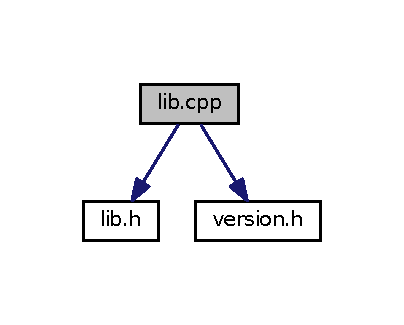
\includegraphics[width=194pt]{lib_8cpp__incl}
\end{center}
\end{figure}
\subsection*{Functions}
\begin{DoxyCompactItemize}
\item 
int \hyperlink{lib_8cpp_ae64f17a84dc9c7144d1036498ff26fd9}{version} ()
\end{DoxyCompactItemize}


\subsection{Function Documentation}
\index{lib.\+cpp@{lib.\+cpp}!version@{version}}
\index{version@{version}!lib.\+cpp@{lib.\+cpp}}
\subsubsection[{\texorpdfstring{version()}{version()}}]{\setlength{\rightskip}{0pt plus 5cm}int version (
\begin{DoxyParamCaption}
{}
\end{DoxyParamCaption}
)}\hypertarget{lib_8cpp_ae64f17a84dc9c7144d1036498ff26fd9}{}\label{lib_8cpp_ae64f17a84dc9c7144d1036498ff26fd9}

\hypertarget{lib_8h}{}\section{lib.\+h File Reference}
\label{lib_8h}\index{lib.\+h@{lib.\+h}}
This graph shows which files directly or indirectly include this file\+:
\nopagebreak
\begin{figure}[H]
\begin{center}
\leavevmode
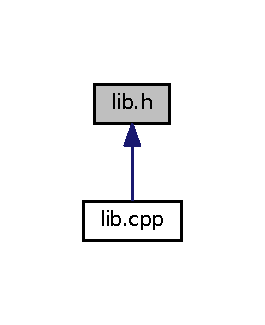
\includegraphics[width=127pt]{lib_8h__dep__incl}
\end{center}
\end{figure}
\subsection*{Functions}
\begin{DoxyCompactItemize}
\item 
int \hyperlink{lib_8h_ae64f17a84dc9c7144d1036498ff26fd9}{version} ()
\end{DoxyCompactItemize}


\subsection{Function Documentation}
\index{lib.\+h@{lib.\+h}!version@{version}}
\index{version@{version}!lib.\+h@{lib.\+h}}
\subsubsection[{\texorpdfstring{version()}{version()}}]{\setlength{\rightskip}{0pt plus 5cm}int version (
\begin{DoxyParamCaption}
{}
\end{DoxyParamCaption}
)}\hypertarget{lib_8h_ae64f17a84dc9c7144d1036498ff26fd9}{}\label{lib_8h_ae64f17a84dc9c7144d1036498ff26fd9}

\hypertarget{version_8h}{}\section{version.\+h File Reference}
\label{version_8h}\index{version.\+h@{version.\+h}}
This graph shows which files directly or indirectly include this file\+:
\nopagebreak
\begin{figure}[H]
\begin{center}
\leavevmode
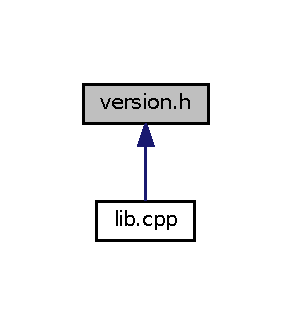
\includegraphics[width=140pt]{version_8h__dep__incl}
\end{center}
\end{figure}
\subsection*{Macros}
\begin{DoxyCompactItemize}
\item 
\#define \hyperlink{version_8h_a4a5fc96a4bdd7d68ed99ccce9ca2e77e}{P\+R\+O\+J\+E\+C\+T\+\_\+\+V\+E\+R\+S\+I\+O\+N\+\_\+\+P\+A\+T\+CH}~3
\end{DoxyCompactItemize}


\subsection{Macro Definition Documentation}
\index{version.\+h@{version.\+h}!P\+R\+O\+J\+E\+C\+T\+\_\+\+V\+E\+R\+S\+I\+O\+N\+\_\+\+P\+A\+T\+CH@{P\+R\+O\+J\+E\+C\+T\+\_\+\+V\+E\+R\+S\+I\+O\+N\+\_\+\+P\+A\+T\+CH}}
\index{P\+R\+O\+J\+E\+C\+T\+\_\+\+V\+E\+R\+S\+I\+O\+N\+\_\+\+P\+A\+T\+CH@{P\+R\+O\+J\+E\+C\+T\+\_\+\+V\+E\+R\+S\+I\+O\+N\+\_\+\+P\+A\+T\+CH}!version.\+h@{version.\+h}}
\subsubsection[{\texorpdfstring{P\+R\+O\+J\+E\+C\+T\+\_\+\+V\+E\+R\+S\+I\+O\+N\+\_\+\+P\+A\+T\+CH}{PROJECT_VERSION_PATCH}}]{\setlength{\rightskip}{0pt plus 5cm}\#define P\+R\+O\+J\+E\+C\+T\+\_\+\+V\+E\+R\+S\+I\+O\+N\+\_\+\+P\+A\+T\+CH~3}\hypertarget{version_8h_a4a5fc96a4bdd7d68ed99ccce9ca2e77e}{}\label{version_8h_a4a5fc96a4bdd7d68ed99ccce9ca2e77e}

%--- End generated contents ---

% Index
\backmatter
\newpage
\phantomsection
\clearemptydoublepage
\addcontentsline{toc}{chapter}{Index}
\printindex

\end{document}
